\documentclass[a4paper, 12pt]{article}
\usepackage[utf8]{inputenc}
\DeclareUnicodeCharacter{2074}{\ensuremath{{}^4}}
\usepackage{listings}
\usepackage{graphicx}
\title{Obligatorisk innlevering 2}
\author{Sivert M. Skarning}
\date{Mai 2019}
\begin{document}
\maketitle

\section{Oppgave 1}
\subsection{Oppgavebeskrivelse}
Implementere DFT og IDFT på egen hånd. Algoritmene skal implementeres slik som gitt i boka, hvis ikke annet er tydelig dokumentert i egen rapport. Algoritmenes korrekthet skal demonstreres på enkle bilder.

\subsection{Dokumentasjon}
I oppgave 1 har jeg laget et skript som tar inn et valgt bilde og fouriertransformerer og invers-fouriertransformerer et bilde både med innebygde funksjoner og med egenskrevne funksjoner. De egenskrevne funksjonene er har en effektivitet på $O(n⁴)$. De er følgelig veldig trege for de store bildene. Dette gjør at bildene jeg har brukt er veldig små.
\subsection{Resultat}
Som et eksempel bilde valgte jeg en 30x30 bilde av et rektangel. For å teste at implementasjonen mine fungerer, bruker jeg fft pack sine funkjsoner for å gjøre samme transformasjon. Man ser følgelig at figur \ref{fig:fft} er lik \ref{fig:dft} og at figur \ref{fig:ifft} er lik \ref{fig:idft}. Dette vil si at implementasjonen skal fungere. Vist man observerer figur \ref{fig:dft} ser vi at det er to retninger som dominerer. Den sterkeste retningen er den horisontale retningen. Fordi oppløsningen er så dårlig ser vi at det vil danne seg overgagner i intensitet på det spatiale bilde i vertikal retning. Det er derfor vi får flere linjer i horisontal retning i det fouriertransformerte bilde. 


\begin{figure}[h]
  \centering
  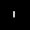
\includegraphics[width=0.5\textwidth]{images/rektangel.png}
  \caption{Rektangel i spatialt domene}
  \label{fig:rektangel}
\end{figure}


\begin{figure}[h]
  \centering
  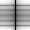
\includegraphics[width=0.5\textwidth]{images/fftpack-rektangel}
  \caption{Rektangel i frekvensdomene, FFT pack}
  \label{fig:fft}
\end{figure}


\begin{figure}[h]
  \centering
  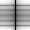
\includegraphics[width=0.5\textwidth]{images/myfft-rektangel}
  \caption{Rektangel i frekvensdomene, egenimplementert dft funksjon}
  \label{fig:dft}
\end{figure}


\begin{figure}[h]
  \centering
  
\includegraphics[width=0.5\textwidth]{images/ifft-rektangel}
  \caption{Rektangel i det spatiale domene(ifft)}
  \label{fig:ifft}
\end{figure}


\begin{figure}[h]
  \centering
  
\includegraphics[width=0.5\textwidth]{images/idft-rektangel}
  \caption{Rektangel i det spatiale domene, egenimplementert idft funksjon}
  \label{fig:idft}
\end{figure}



\end{document}